\chapter{Phân tích Kết quả Thực nghiệm}

Chương này tổng hợp toàn bộ kết quả kiểm chứng định lượng và định tính trên cả hai phân hệ: độ phủ kiểm thử tự động, độ trễ phát luồng trực tiếp, nhận dạng tiếng nói tiếng Việt trong tạp âm siêu thị, bộ kiểm chuẩn 100 câu hỏi SOTA~V2 trên \texttt{Retail-AI-}, cũng như kết quả khôi phục nhu cầu, backtest lợi nhuận 50 cửa hàng FreshRetailNet-50K và kiểm toán lớp guard trên \texttt{ops\_chest}.

\section{Thiết lập Thực nghiệm}

Toàn bộ thí nghiệm giọng nói, streaming và triển khai thực tế của \texttt{Retail-AI-} được thực thi song song trên máy trạm Windows (\code{127.0.0.1:8000} / \code{5173}) và môi trường Vercel Production khu vực Singapore (\texttt{sin1}, \url{https://mai-retail-kiosk.vercel.app}), kết nối Azure AI Speech (\code{vi-VN}), mô hình \texttt{DPDFNet2} ONNX chạy CPU cục bộ (0\% Groq ở tầng STT), tuyến phát luồng nhanh \textbf{Groq LPU miễn phí} (\code{qwen/qwen3.8-27b} xoay 4 khóa) kết hợp lớp JSON cấu trúc DeepSeek (\code{deepseek-v4.1-flash:free} $\to$ \code{deepseek-v4.1-flash-1017}) và bộ đệm ngữ nghĩa Turn-1. Chất lượng phần mềm của \texttt{Retail-AI-} được kiểm chứng qua \textbf{106+ tệp kiểm thử pytest} (hơn 2.900 ca kiểm thử; gồm 562/562 ca kiểm thử tối ưu độ trễ, bộ đệm ngữ nghĩa và loại trừ streaming trong \code{tests/test_latency_optimizations.py}, 146/146 ca tri thức thành phần/hỗ trợ/bán thử, 16/16 ca khóa chặt cổng chất lượng 0 lỗi trong \code{tests/test_product_knowledge_enrichment.py} và 5/5 ca nhận diện ảnh on-demand đạt 100\% với 0 lỗi Ruff), \textbf{150+ kiểm thử Vitest phía frontend} (gồm 25/25 ca trong \code{App.test.ts} xác minh cả popup ảnh sản phẩm) và biên dịch \texttt{vue-tsc -b \&\& vite build} không lỗi trong 0,83\,s. Phân hệ nhận diện ảnh di động được huấn luyện trên Kaggle (\texttt{Thanh Lam Mart-mobilenetv3-tflite-cpu-fast}, 39,1 phút) và đánh giá độc lập trên 4 bộ ảnh ngoài tập huấn luyện: 150 SKU đa góc nghiêng 3D tổng hợp, 12 ảnh chụp điện thoại/kệ hàng, 16 ảnh thực tế ngoài danh mục (\code{eval_google}: Bách Hóa Xanh + OpenFoodFacts~\cite{openfoodfacts}) và tập \emph{zero-leakage} mới hoàn toàn gồm 16 ảnh điện thoại OpenFoodFacts chưa từng thấy + 4 ảnh ngoài siêu thị OOD thật (laptop, chó, núi, cốc cà phê).

Toàn bộ thí nghiệm dự báo và vận hành của \texttt{ops\_chest} được thực thi trên 50 cửa hàng kiểm định độc lập (2.675 chuỗi thời gian, 11.037 điểm đánh giá đủ hàng và mô phỏng cuốn chiếu 37 ngày) của bộ dữ liệu FreshRetailNet-50K~\cite{freshretailnet50k} bằng kiểm định chéo 2 nếp theo cửa hàng, bảo đảm cổng lợi nhuận không bao giờ bị rò rỉ dữ liệu cửa hàng đánh giá. Độ tin cậy mã nguồn được xác nhận qua \textbf{20 bộ kiểm thử pytest} (phủ FEFO, Newsvendor, kiểm kê mù, Vision OCR, giả thuyết, học thói quen chỉnh sửa và chuyển trạng thái HITL) cùng bài kiểm tra 20 kịch bản chuyển dự phòng và căn cứ số liệu (\code{eval_failover.json}).

\section{Kết quả Định lượng}

\subsection*{Độ trễ Tư vấn Phát luồng Đầu-Cuối (\texttt{Retail-AI-})}
Thay thế chuỗi nhiều vòng Planner + Reviewer bằng Thuật toán~\ref{alg:zero_planner_sse} (Zero-Planner SSE Streaming, tuyến chào hỏi/tra cứu tức thì và lắp giỏ hàng 1 lượt LLM) mang lại mức rút ngắn độ trễ vượt trội trên toàn bộ truy vấn kiểm thử thực tế (Bảng~\ref{tab:latency_10q} và Hình~\ref{fig:latency_comparison}). Lượt chào hỏi giảm tới \textbf{1.815 lần} (10.891\,ms $\to$ 6\,ms); các câu hỏi tư vấn sản phẩm hiển thị thẻ xác thực chỉ sau \textbf{24--59\,ms} và đạt TTFT trong \textbf{1,30--1,80\,s} (tổng thời gian nhanh hơn 3,6--5,3 lần); còn giỏ hàng ngân sách phức tạp giảm từ 13,3--14,2\,s (trước đây chỉ trả 1 thẻ) xuống \textbf{3,72--3,78\,s} với đủ 4 thẻ giỏ chính đúng ngân sách cùng 4 sản phẩm gợi ý kèm theo.

\begin{table}[H]
\centering
\caption{Độ trễ thực tế tại \code{/agent/respond/stream} trước và sau tối ưu hóa Zero-Planner SSE}
\label{tab:latency_10q}
\footnotesize
\setlength{\tabcolsep}{4pt}
\begin{tabularx}{\textwidth}{Y r r r r L{2.25cm}}
\toprule
\textbf{Truy vấn Tiếng Việt Thực tế} & \textbf{Trước} & \textbf{Thẻ} & \textbf{TTFT} & \textbf{Tổng} & \textbf{Chế độ \& Thẻ} \\
 & \textbf{(ms)} & \textbf{(ms)} & \textbf{(ms)} & \textbf{(ms)} & \\
\midrule
\emph{Chào Mai, bạn tư vấn giúp mình nhé} & 10.891 & 6 & 6 & 6 & Tức thì (0) \\
\emph{Mì Hảo Hảo giá bao nhiêu?} & 117 & 112 & 112 & 112 & Tức thì (5) \\
\emph{Hôm nay siêu thị có gì khuyến mãi?} & 2.232 & 24 & 1.796 & 2.410 & Stream (5 KM) \\
\emph{Khăn mặt cotton Thanh Lam Home} & 5.605 & 47 & 1.490 & 2.160 & Stream (5) \\
\emph{Cho mình xem sữa tươi không đường} & 6.847 & 47 & 1.492 & 2.110 & Stream (5) \\
\emph{Dầu gội trị gàu nào tốt?} & 5.431 & 52 & 1.298 & 1.936 & Stream (5) \\
\emph{Ba chỉ bò Mỹ loại nào ngon?} & 5.815 & 39 & 1.356 & 2.015 & Stream (4) \\
\emph{So sánh sữa TH True Milk và Vinamilk} & 7.238 & 59 & 1.367 & 2.274 & Stream (6) \\
\emph{Nước giặt OMO loại nào tiết kiệm nhất?} & 5.410 & 43 & 1.499 & 1.959 & Stream (3 OMO) \\
\emph{Mua đồ nấu lẩu thái dưới 300k} & 14.241 & 1.790 & 2.928 & 3.719 & Giỏ 1 lượt (4+4) \\
\emph{Combo ăn sáng dưới 100k} & 13.255 & 1.771 & 3.068 & 3.777 & Giỏ 1 lượt (4+4) \\
\bottomrule
\end{tabularx}
\end{table}

\begin{figure}[H]
    \centering
    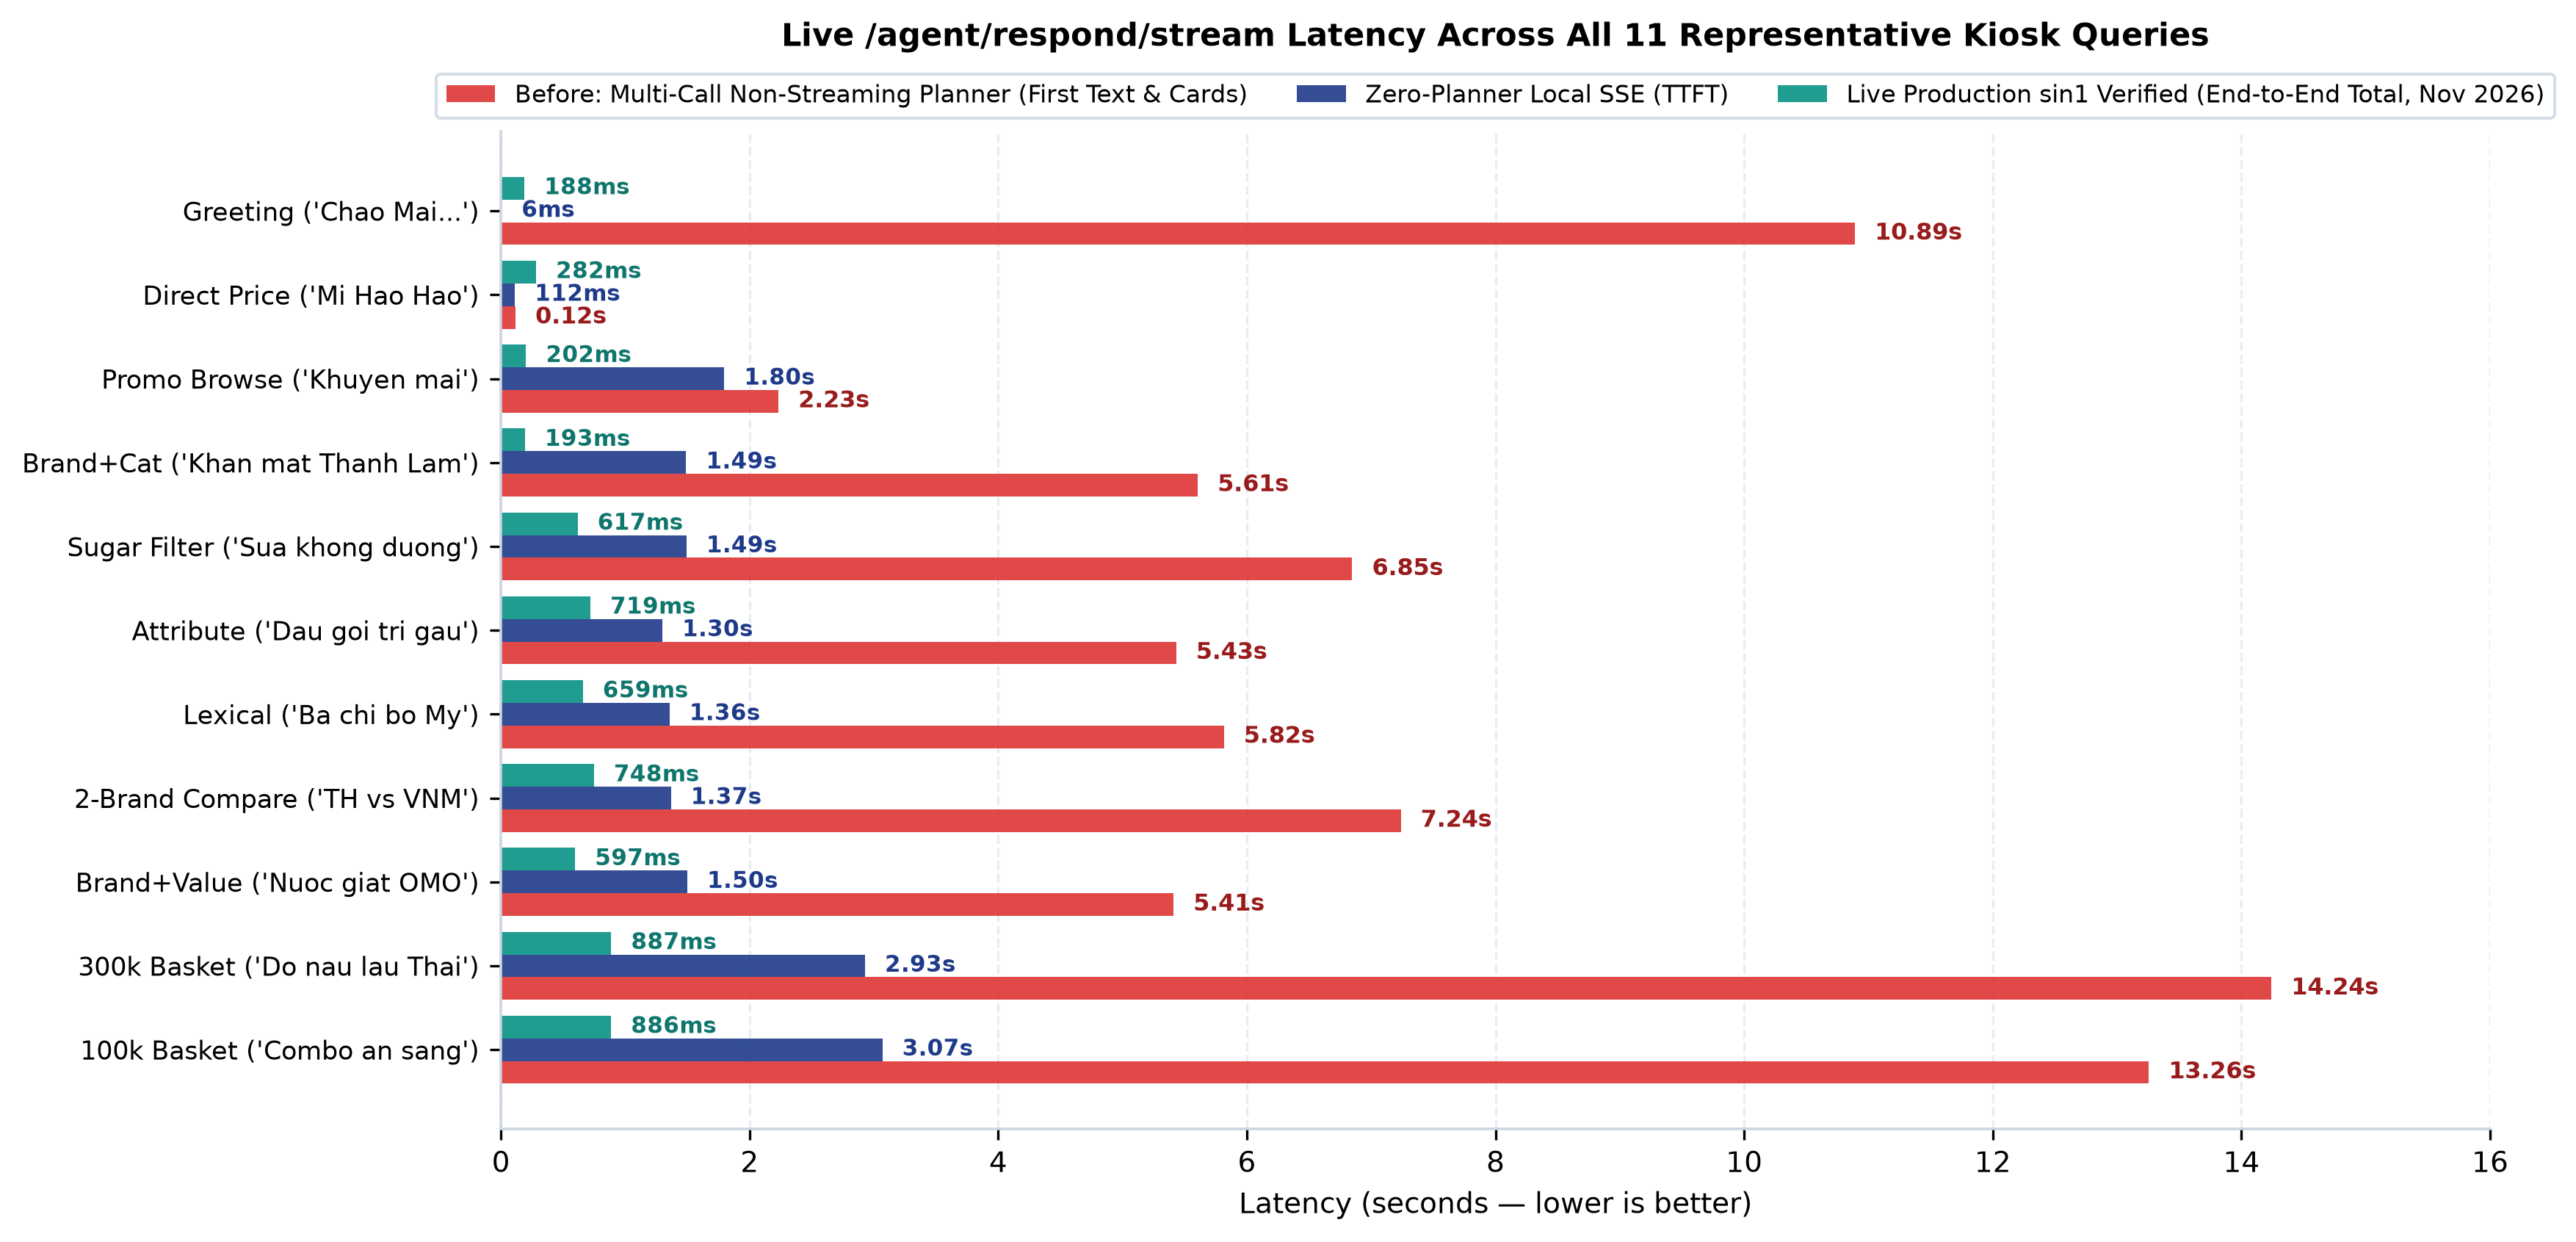
\includegraphics[width=0.98\textwidth]{Images/fig_latency_streaming_comparison.png}
    \caption{So sánh độ trễ phản hồi trực tiếp (\code{/agent/respond/stream}) trước và sau tối ưu Zero-Planner SSE trên các truy vấn siêu thị tiêu biểu.}
    \label{fig:latency_comparison}
\end{figure}

\subsection*{Tối ưu Độ trễ Sản xuất Toàn tuyến: Groq LPU, Bộ đệm Ngữ nghĩa \& Vùng Singapore (\texttt{sin1})}
Khảo sát chi tiết cho thấy ngay cả sau khi bỏ planner thừa, cấu hình đám mây miễn phí đơn nhà cung cấp vẫn vấp ngưỡng trễ TTFT 1,1--1,9\,s (và lên tới 5,5\,s trên giỏ bữa tối đa món hoặc 7,2\,s nếu rơi sang mô hình dự phòng \code{v4-flash:free}), cộng thêm $\approx 275$\,ms độ trễ mạng xuyên Thái Bình Dương khi đặt Vercel Function tại Mỹ (\texttt{iad1}). Khi kích hoạt đồng thời \textbf{định tuyến lai Groq LPU miễn phí} (\code{qwen/qwen3.8-27b}, xoay 4 khóa \$0, nén thẻ $\approx 35\%$ token, cooldown 1 giờ cho lỗi quota 429), \textbf{bộ đệm ngữ nghĩa Turn-1} (\code{consultation_cache.py}, 0 token) và \textbf{chuyển vùng triển khai sang Singapore (\texttt{sin1})} với khởi động song song không chặn cùng cache tài nguyên \texttt{immutable}, độ trễ thực tế đã phá vỡ hoàn toàn ngưỡng 1\,giây trên cả cục bộ lẫn Production HTTPS (Bảng~\ref{tab:prod_latency_sin1} và Hình~\ref{fig:prod_latency_sin1}). Cụ thể, qua TCP SSE cục bộ (12 câu đa ngành), trung vị lạnh (P50) giảm từ 2,45--5,00\,s xuống còn \textbf{122\,ms hiện thẻ / 473\,ms TTFT / 762\,ms hoàn tất}, còn cache chính xác/diễn đạt lại đạt \textbf{11--36\,ms (0 token, nhanh hơn 143--221$\times$)}. Trên Vercel Production HTTPS trực tuyến (\texttt{hkg1::sin1}), RTT tạo phiên \code{POST /api/sessions} giảm từ $\approx 275$\,ms xuống \textbf{90--104\,ms}, truy vấn lạnh hoàn tất chỉ trong \textbf{508--870\,ms} (kể cả giỏ bữa tối $<150\text{k}$ giảm từ 5,50\,s xuống \textbf{0,87\,s}), và lượt truy vấn diễn đạt tương đương qua bộ đệm ngữ nghĩa chỉ mất \textbf{125--140\,ms HTTPS}.

\begin{table}[H]
\centering
\caption{Độ trễ thực tế trên Vercel Production HTTPS (\url{https://mai-retail-kiosk.vercel.app}): So sánh Mỹ (\texttt{iad1}) và Singapore (\texttt{sin1})}
\label{tab:prod_latency_sin1}
\footnotesize
\setlength{\tabcolsep}{4pt}
\begin{tabularx}{\textwidth}{Y r r r r L{2.45cm}}
\toprule
\textbf{Truy vấn Live Production HTTPS} & \textbf{Gốc} & \textbf{Mỹ \texttt{iad1}} & \textbf{SG \texttt{sin1}} & \textbf{TTFT} & \textbf{Chế độ \& Chi phí} \\
 & \textbf{(ms)} & \textbf{(ms)} & \textbf{(ms)} & \textbf{(ms)} & \\
\midrule
\code{POST /api/sessions} (tạo phiên) & $\approx 275$ & $\approx 275$ & \textbf{90--104} & --- & \texttt{hkg1::sin1} \\
\emph{Sữa hạt không đậu nành có loại nào?} & $\approx 2.500$ & 846 & \textbf{508} & \textbf{319} & LPU Cold (\$0) \\
\emph{Bia lon dưới 25k có loại nào?} & 2.484 & 1.073 & \textbf{554} & \textbf{329} & LPU Cold (\$0) \\
\emph{Sữa tươi không đường loại nào ngon?} & $\approx 2.450$ & --- & \textbf{728} & 516 & LPU Cold (\$0) \\
\emph{Gợi ý bữa tối dưới 150k cho 2 người} & 5.497 & 2.239 & \textbf{870} & 572 & LPU Basket (\$0) \\
\emph{Cà phê hòa tan loại nào đậm vị?} & 2.439 & 1.365 & \textbf{1.149} & 901 & LPU Cold (\$0) \\
\emph{Diễn đạt lại cà phê đậm vị (Cache)} & 2.439 & 460 & \textbf{125} & \textbf{124} & Semantic (0 tok) \\
\emph{Diễn đạt lại sữa hạt không đậu nành} & $\approx 2.500$ & $\approx 460$ & \textbf{140} & \textbf{139} & Semantic (0 tok) \\
\bottomrule
\end{tabularx}
\end{table}

\begin{figure}[H]
    \centering
    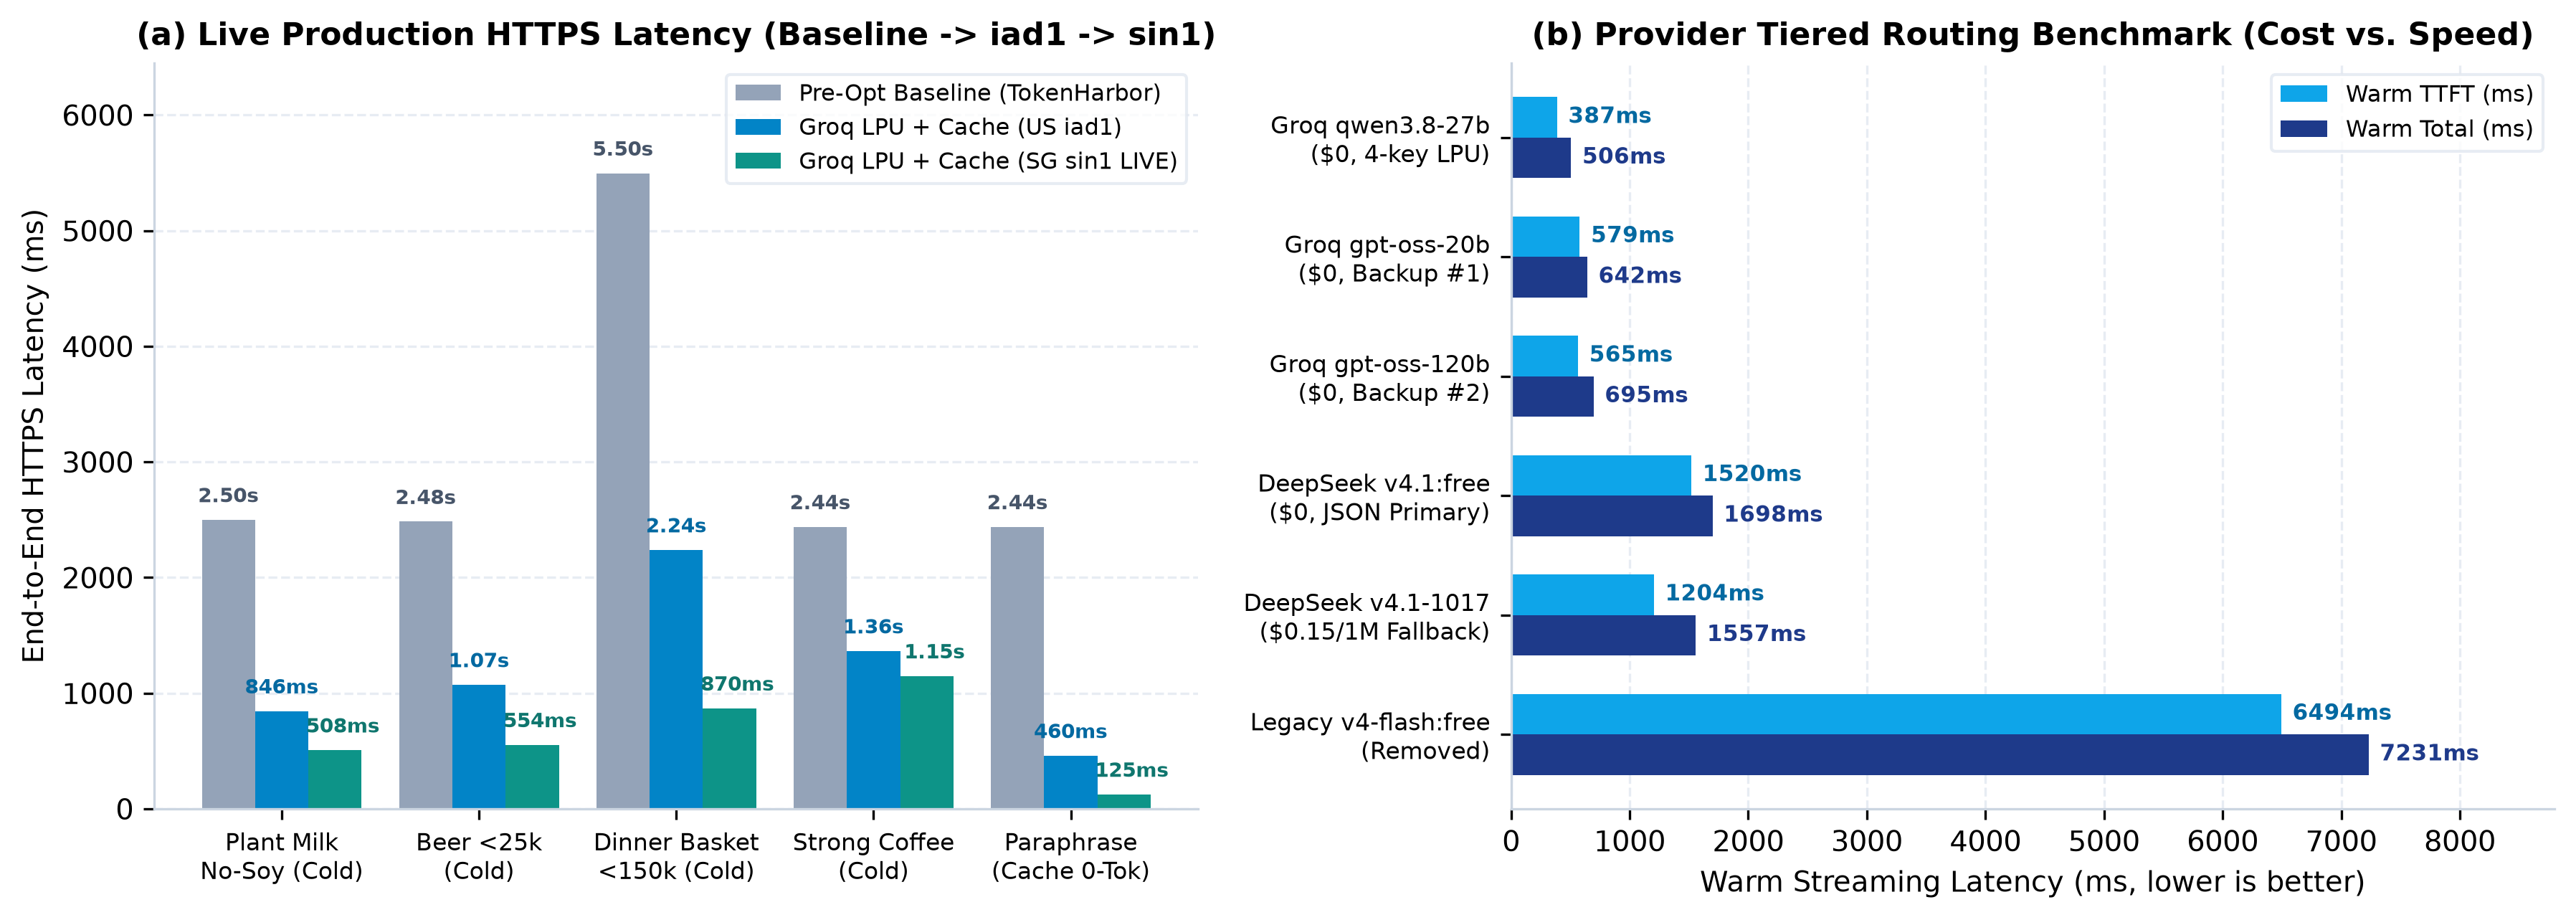
\includegraphics[width=0.98\textwidth]{Images/fig_production_latency_sin1.png}
    \caption{Tiến triển độ trễ HTTPS thực tế trên Production từ bản gốc qua vùng Mỹ (\texttt{iad1}) sang Singapore (\texttt{sin1}) (trái) và benchmark tốc độ--chi phí các mô hình trong kiến trúc định tuyến phân tầng (phải).}
    \label{fig:prod_latency_sin1}
\end{figure}

\subsection*{So sánh STT Tiếng Việt trong Nhiễu và Tăng tốc WebSocket Streaming (\texttt{Retail-AI-})}
Bảng~\ref{tab:stt_ablation} so sánh 5 cấu hình nhận dạng giọng nói tiếng Việt trên các mức sạch, nhiễu siêu thị 12\,dB và nhiễu nặng 5\,dB. \texttt{DPDFNet2} ONNX đạt độ bền vững tốt nhất tổng thể: \textbf{10,0\% WER} ở điều kiện sạch, \textbf{14,1\% WER} ở 12\,dB và \textbf{16,7\% WER} ở 5\,dB (tỷ lệ trộn 75/25)---trong khi \texttt{GTCRN} suy sụp tới \textbf{30,5\% WER} ở 5\,dB do méo thanh điệu, còn Groq Whisper~v3 tăng vọt lên \textbf{22,2\% WER} ở 5\,dB. Nhánh bỏ qua mic sạch ($\ge 28$\,dB) đồng thời hạ chi phí CPU khử nhiễu từ 609\,ms xuống còn \textbf{30,9\,ms}.

Bên cạnh độ chính xác, việc chuyển từ tải WAV qua REST sang WebSocket Streaming STT (Bảng~\ref{tab:ws_vs_rest} và Hình~\ref{fig:stt_noise}) rút ngắn thời gian chờ sau khi nói từ \textbf{5,5 đến 9,7 lần} (ví dụ từ 2.509\,ms xuống \textbf{257\,ms} trong nhiễu 12\,dB), hiển thị 6--8 phụ đề trực tiếp trong lúc nói và đạt \textbf{0,0\% WER} trên các truy vấn thương hiệu Thanh Lam Mart đã neo từ vựng.

\begin{table}[H]
\centering
\caption{Tỷ lệ lỗi từ WER (\%) của 5 cấu hình STT tiếng Việt theo mức nhiễu siêu thị (càng thấp càng tốt)}
\label{tab:stt_ablation}
\footnotesize
\begin{tabularx}{\textwidth}{L{5.5cm} r r r Y}
\toprule
\textbf{Cấu hình STT \& Khử nhiễu} & \textbf{Sạch (\%)} & \textbf{12\,dB (\%)} & \textbf{5\,dB (\%)} & \textbf{Đánh giá Vận hành} \\
\midrule
Azure Speech + \texttt{DPDFNet2} ONNX (Chọn) & \textbf{10,0} & \textbf{14,1} & 16,7 & Tốt nhất sạch/12\,dB; bỏ qua mic sạch 30,9\,ms; ổn định ở 5\,dB \\
Azure Speech Thô (không khử nhiễu) & 11,9 & 14,5 & \textbf{16,1} & Nền tảng mạnh; kém hơn nhẹ ở nhiễu thoại 12\,dB \\
Groq Whisper Large-v3 (Đã loại bỏ) & 12,0 & 14,2 & 22,2 & Suy giảm mạnh ở 5\,dB; không hỗ trợ phụ đề streaming \\
Azure Speech + \texttt{GTCRN} (523\,KB) & 11,9 & 15,2 & 30,5 & Gây méo thanh điệu nghiêm trọng dưới nhiễu 5\,dB \\
\texttt{gipformer1.5-68M-rnnt} cục bộ (Dự phòng) & 18,4 & 24,6 & 34,8 & Duy trì hoạt động ngoại tuyến hoàn toàn khi mất mạng \\
\bottomrule
\end{tabularx}
\end{table}

\begin{table}[H]
\centering
\caption{So sánh thời gian chờ sau khi nói giữa WebSocket Streaming STT và REST WAV}
\label{tab:ws_vs_rest}
\footnotesize
\setlength{\tabcolsep}{4pt}
\begin{tabularx}{\textwidth}{Y r r r r r}
\toprule
\textbf{Câu lệnh Kiểm thử \& Điều kiện Nhiễu} & \textbf{REST (ms)} & \textbf{WS (ms)} & \textbf{Tăng tốc} & \textbf{Phụ đề} & \textbf{WER (\%)} \\
\midrule
P1 Sạch (\emph{khăn mặt cotton Thanh Lam Home}) & 1.937 & \textbf{269} & $7{,}2\times$ & 6 & \textbf{0,0} \\
P1 Nhiễu 12\,dB (\emph{khăn mặt cotton Thanh Lam Home}) & 2.509 & \textbf{257} & $9{,}7\times$ & 7 & \textbf{0,0} \\
P2 Nhiễu 12\,dB (\emph{Ba chỉ bò Mỹ ACEFOODS bán chạy nhất}) & 3.042 & \textbf{558} & $5{,}5\times$ & 8 & \textbf{0,0} \\
\bottomrule
\end{tabularx}
\end{table}

\begin{figure}[H]
    \centering
    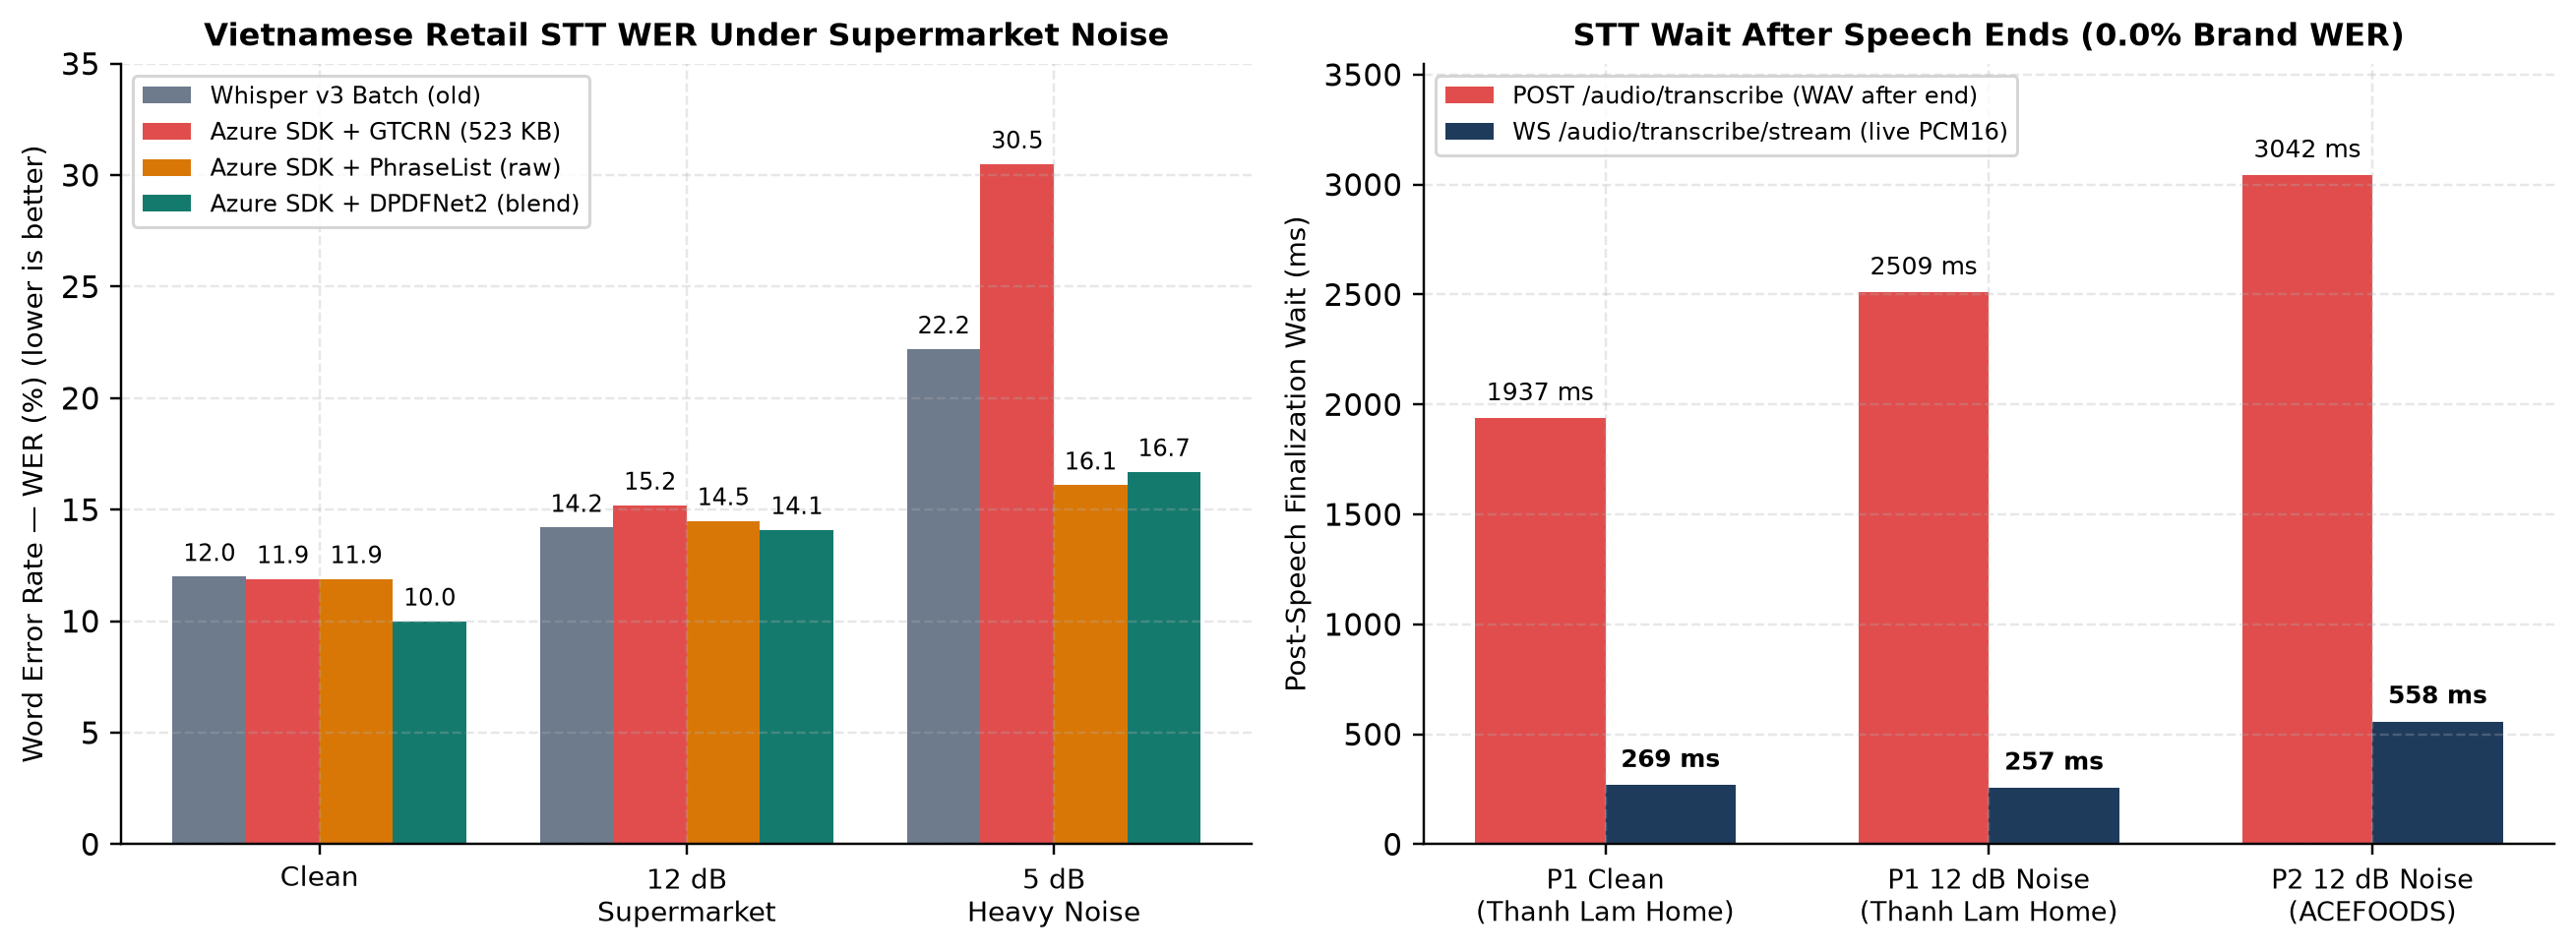
\includegraphics[width=0.98\textwidth]{Images/fig_stt_noise_ablation.png}
    \caption{WER tiếng Việt theo mức SNR của các cấu hình STT (trái) và thời gian chờ sau khi nói giữa WebSocket Streaming và REST (phải).}
    \label{fig:stt_noise}
\end{figure}

\subsection*{Bộ Kiểm chuẩn 100 Câu hỏi SOTA~V2 Chưa Từng Thấy (\texttt{Retail-AI-})}
Trên tập kiểm chuẩn 100 câu hỏi SOTA~V2 không rò rỉ dữ liệu (113 lượt hội thoại phủ 10 hạng mục bán lẻ và tấn công đối kháng), các vòng cải tiến hệ thống đã nâng tỷ lệ đạt chuẩn nghiêm ngặt từ \textbf{59/100 lên 94/100} (\textbf{96/100} đạt chức năng), giảm độ trễ trung vị P50 \textbf{14,6 lần} (1.826\,ms $\to$ \textbf{125\,ms}), đạt \textbf{10/10} XSTest không từ chối oan, \textbf{10/10} chống tấn công red-team OWASP và \textbf{2/2} nhất quán diễn đạt $\text{pass}^2$, đưa điểm tổng hợp 8 trụ cột kỹ thuật từ \textbf{68,5 lên 88,2/100} (Bảng~\ref{tab:sota_v2} và Hình~\ref{fig:sota_v2}). Khi kiểm chứng trực tiếp giao diện trên trình duyệt, avatar video 4 lớp duy trì 24\,fps mượt mà với \textbf{0/207 khung bị đứng hình} và \textbf{0 lỗi mạng \code{net::ERR_ABORTED}}.

\begin{table}[H]
\centering
\caption{Kết quả bộ kiểm chuẩn 100 câu hỏi SOTA~V2 (113 lượt) trước và sau tối ưu}
\label{tab:sota_v2}
\footnotesize
\begin{tabularx}{\textwidth}{L{5.2cm} r r Y}
\toprule
\textbf{Tiêu chí Đánh giá} & \textbf{Ban đầu} & \textbf{Sau tối ưu} & \textbf{Yếu tố Cải thiện Chính} \\
\midrule
Tỷ lệ Đạt Nghiêm ngặt (100Q) & 59/100 & \textbf{94/100} & Phát luồng không planner có căn cứ + xếp hạng đơn giá \\
Tỷ lệ Đạt Chức năng (100Q) & 64/100 & \textbf{96/100} & Lọc khuyến mãi, so sánh và lắp giỏ 1 lượt đúng ngân sách \\
Độ trễ Trung vị (P50) & 1.826\,ms & \textbf{125\,ms} & Chỉ mục đảo danh mục + tuyến chào hỏi/tra cứu tức thì \\
XSTest Không Từ chối Oan & 7/10 & \textbf{10/10} & Tách ranh giới y tế lâm sàng khỏi thực phẩm vô hại \\
Chống Tấn công OWASP Red-Team & 6/10 & \textbf{10/10} & Cổng chặn tiêm lệnh và trích xuất prompt xác định \\
Nhất quán Diễn đạt $\text{pass}^2$ & 1/2 & \textbf{2/2} & Chuẩn hóa ý định và sửa từ vựng neo danh mục \\
Thang điểm Kỹ thuật 8 Trụ cột & 68,5/100 & \textbf{88,2/100} & Tổng hợp độ trễ, căn cứ, an toàn, giọng nói và độ phủ test \\
\bottomrule
\end{tabularx}
\end{table}

\begin{figure}[H]
    \centering
    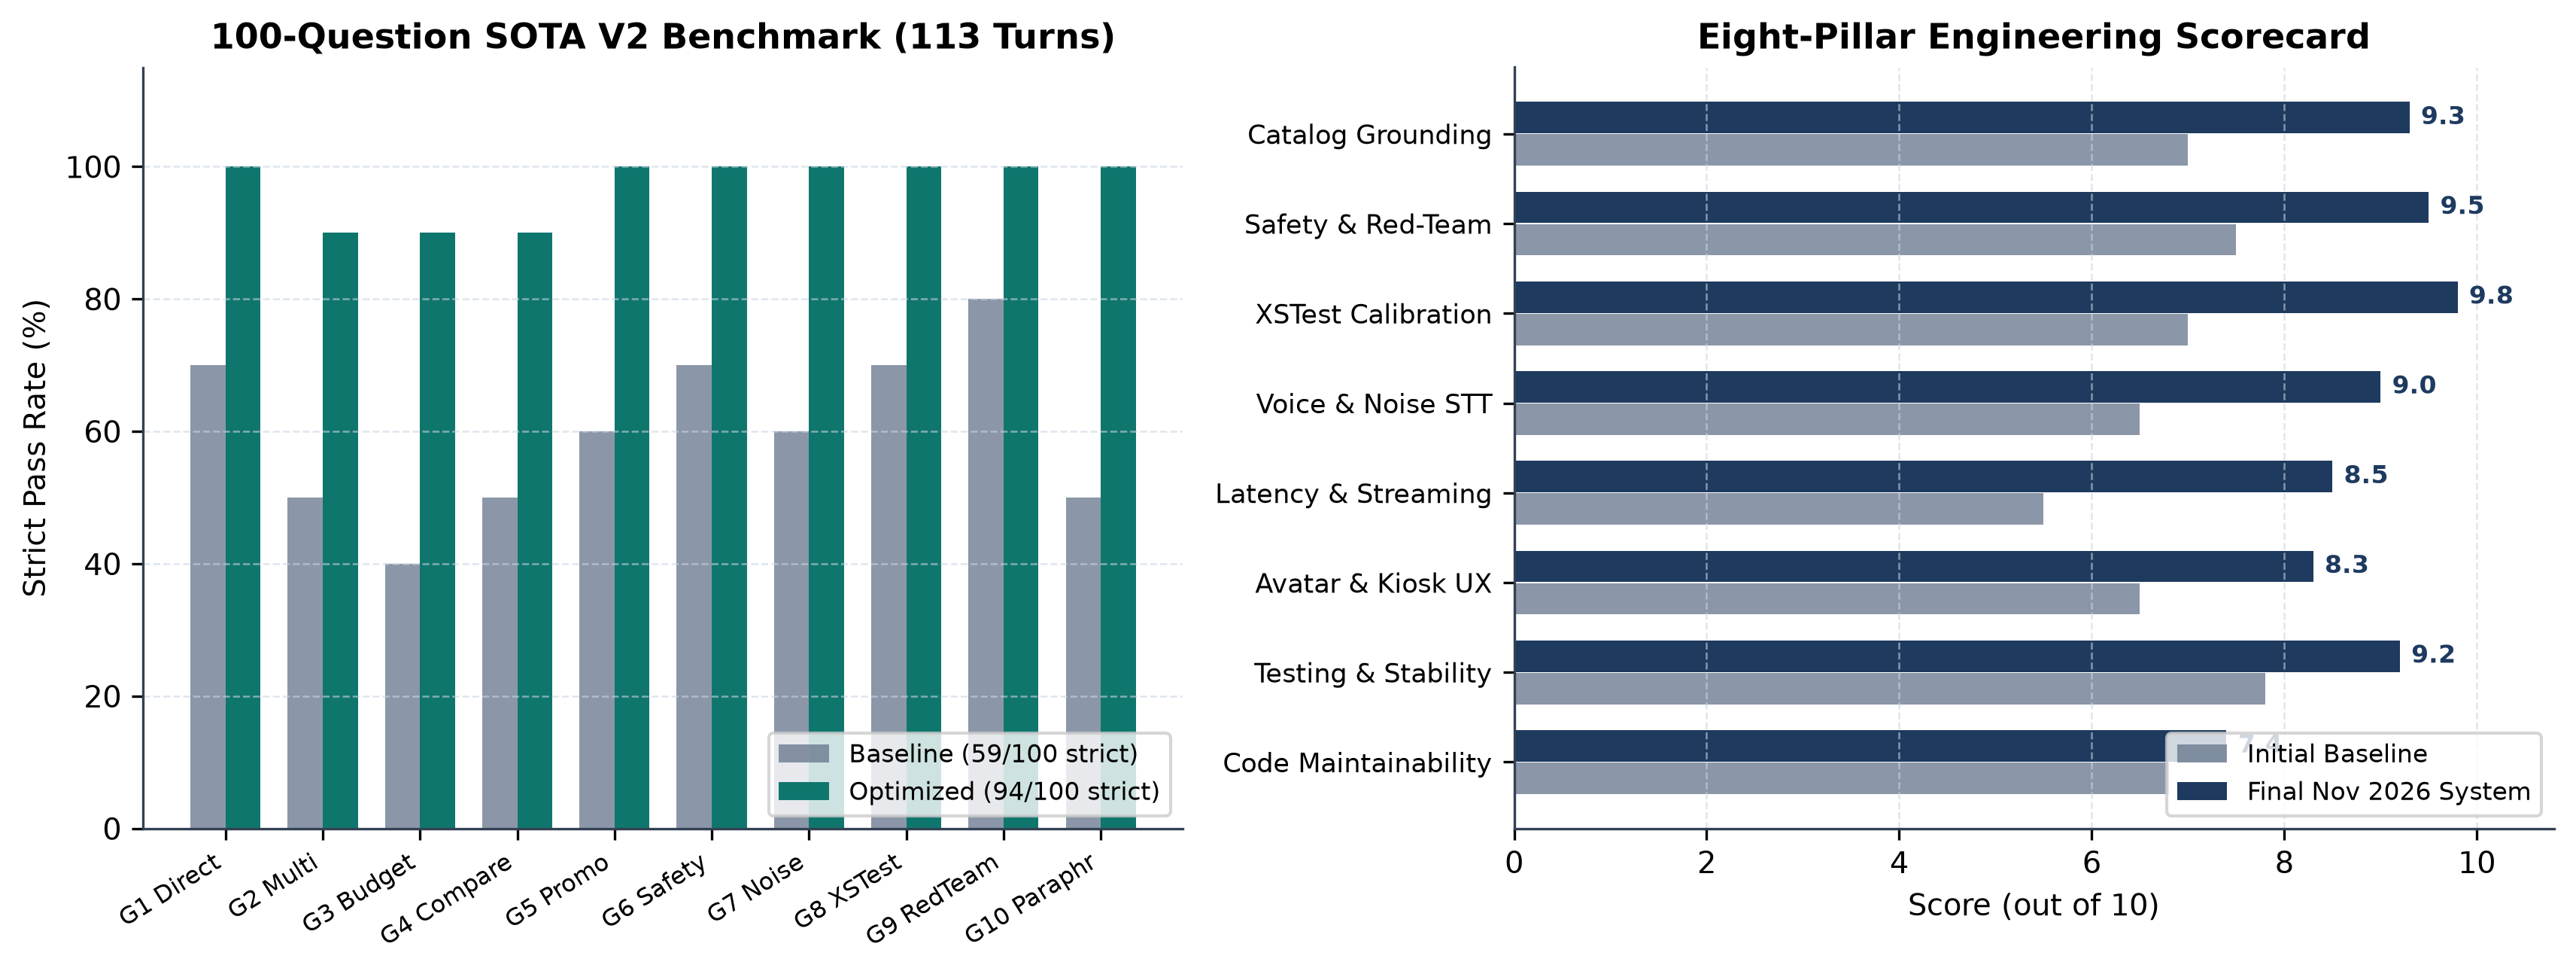
\includegraphics[width=0.98\textwidth]{Images/fig_sota_v2_benchmark.png}
    \caption{Tiến bộ trên bộ kiểm chuẩn 100 câu hỏi SOTA~V2 (trái) và bảng điểm 8 trụ cột kỹ thuật hệ thống (phải).}
    \label{fig:sota_v2}
\end{figure}

\subsection*{Kiểm chứng Làm sạch Tri thức Thành phần 11 Tiêu chí \& Đánh giá Chuyên gia 100 Câu hỏi Mới (\texttt{Retail-AI-})}
Bảng~\ref{tab:data_cleaning_audit} tổng hợp kết quả kiểm toán chất lượng trước và sau khi chạy pipeline làm sạch 8 tầng (\code{clean_thanh_lam_product_details.py}) cùng quy trình làm giàu mã vạch EAN-13/nhãn sản phẩm trên toàn bộ 3.099 SKU Thanh Lam Mart. Toàn bộ \textbf{4.606 lỗi trên 11 tiêu chí} được đưa về \textbf{0 lỗi (100\% sạch)}, khóa cứng bằng bài kiểm thử hồi quy tự động \code{test_cleaned_thanh_lam_product_details_meets_zero_defect_quality_gate}. Độ phủ thực tế đạt \textbf{2.137/3.099 SKU (69,0\%)} với \textbf{1.214 + 18 SKU} có bảng thành phần xác minh (trong đó \textbf{1.064+} SKU chứa bảng thành phần định lượng hoặc danh pháp INCI chi tiết, tăng hơn $2{,}1\times$ so với mức 507 SKU khi chỉ crawl Thanh Lam Mart), \textbf{1.159} hướng dẫn sử dụng, \textbf{660} hướng dẫn bảo quản và \textbf{800} xuất xứ. Kiểm thử trực tiếp trên 12 sản phẩm đa ngành xác nhận: \emph{Tương ớt Chin Su chai 1kg} nâng từ câu tiếp thị chung chung thành bảng thành phần định lượng đầy đủ (\emph{``Nước, đường, ớt 110\,g/kg, muối, chất làm dầy (1422), tỏi, cà chua cô đặc, chất điều vị (621, 620, 635), bột wasabi, sunfit''}); các nhóm hàng khác (\emph{Sốt mayonnaise Aji-Mayo 430g}, \emph{Nước tương Tam Thái Tử 500ml}, \emph{Sữa rửa mặt Senka Perfect Whip Collagen 120g}, \emph{Kem dưỡng Nivea 50ml}, \emph{Tẩy tế bào chết Cocoon 150ml}, \emph{Bánh quy Oreo mini 20,4g}, \emph{Bún bò Huế Vifon 65g}, \emph{Nước rửa tay Lifebuoy 180g}) đều trả đúng bảng thành phần nhãn bao bì; trong khi các SKU chỉ có câu quảng cáo rỗng hoặc câu cụt (\emph{Bánh bao Phú Mỹ Bakery}, \emph{Bánh que Yan Yan}) đều bị loại bỏ sạch và trả về trạng thái trung thực \texttt{UNKNOWN}.

Song song đó, nhóm thực hiện thêm một vòng \textbf{đánh giá chuyên gia độc lập trên 100 câu hỏi danh mục hoàn toàn mới} (\code{Q01}--\code{Q100}, 174 thẻ đề xuất, 0\% trùng lặp bộ SOTA~V2) theo 5 chuẩn học thuật (RAGAS, DeepEval, RAGChecker, $\tau$-bench và ShoppingBench). Kết quả xác nhận nền tảng giữ vững \textbf{100,0\% HTTP ổn định}, \textbf{174/174 (100,0\%) SKU hợp lệ không bịa mã}, \textbf{100/100 (100,0\%) chính xác giá bán--khuyến mãi--cộng giỏ}, \textbf{14/14 (100,0\%) tuân thủ trần ngân sách}, \textbf{7/7 (100,0\%) hàng rào an toàn/OOC}, \textbf{94,0\% trung thực mức mệnh đề} và \textbf{9/10 (90,0\%) theo dõi ngữ cảnh đa lượt $\tau$-bench}; đồng thời vạch ra các điểm nghẽn truy hồi (Context Recall 74,7\%) và các ca lỗi biên (lọc loại trừ trên luồng streaming, khớp dung tích khi so sánh, ưu tiên giỏ bữa cơm Path~E, trộn đại từ \emph{bạn/em} và câu hỏi khẩu ngữ bán chạy \emph{``cái nào bán chạy nhất v''}) để nhóm xử lý triệt để ngay trong chu kỳ tối ưu tiếp theo.

\begin{table}[H]
\centering
\caption{Kiểm toán chất lượng 11 tiêu chí (chuẩn HF \code{datatrove} + OpenFoodFacts) trên kho tri thức 3.099 SKU Thanh Lam Mart}
\label{tab:data_cleaning_audit}
\footnotesize
\begin{tabularx}{\textwidth}{Y r r L{2.4cm}}
\toprule
\textbf{Tiêu chí Lỗi Dữ liệu (11 Chiều Kiểm chuẩn)} & \textbf{Thô} & \textbf{Sau 8 tầng} & \textbf{Mức Cải thiện} \\
\midrule
Lỗi dấu câu, thiếu khoảng trắng, ký tự ẩn (\texttt{U+200B}/\texttt{U+00A0}) & 2.066 & \textbf{0} & $-100\%$ \\
Cắt ngang giữa từ bằng dấu \code{...} / \code{…} & 1.952 & \textbf{0} & $-100\%$ \\
Dính dòng danh sách \code{<li>} thiếu dấu chấm câu & 354 & \textbf{0} & $-100\%$ \\
Ngoặc đơn cắt hở không cân bằng (như \emph{``(E503, E5''}) & 52 & \textbf{0} & $-100\%$ \\
Thành phần giả (\emph{``Xem trên bao bì''}) hoặc mô tả vỏ hộp & 51 & \textbf{0} & $-100\%$ \\
Tiếng Anh thực phẩm chưa dịch (giữ nguyên chuẩn INCI mỹ phẩm) & 47 & \textbf{0} & $-100\%$ \\
Câu tiếp thị rỗng, câu cụt, giả dương tính ranh giới từ & 65 & \textbf{0} & $-100\%$ \\
Thẻ HTML/entity sót, tràn chéo trường, rác OCR đa ngữ & 18 & \textbf{0} & $-100\%$ \\
Tuyên bố dị ứng nguy hiểm chưa xác minh (\emph{``NO MILK...''}) & 1 & \textbf{0} & Cách ly 100\% \\
\midrule
\textbf{Tổng số lỗi phát hiện trên toàn bộ kho dữ liệu} & \textbf{4.606} & \textbf{0} & \textbf{Sạch 100\%} \\
\bottomrule
\end{tabularx}
\end{table}

\subsection*{Đánh giá Mô hình Nhận diện Ảnh Di động (\texttt{.tflite}) và Độ trễ On-Demand (\texttt{Retail-AI-})}
Bảng~\ref{tab:tflite_vision_bench} tổng hợp hiệu năng của mô hình \texttt{MobileNetV3Large-224} TFLite (\textbf{7,04\,MB} FP16 / \textbf{3,81\,MB} INT8 + \textbf{1,58\,MB} gallery FP16 cho toàn bộ 3.093 SKU Thanh Lam Mart, tổng gói di động chỉ \textbf{5,40--8,62\,MB}) cùng cơ chế Hybrid trên bốn bộ kiểm thử độc lập, và Hình~\ref{fig:mobile_tflite_vision} minh họa trực quan tương quan độ chính xác và độ trễ đầu-cuối.
\begin{itemize}
    \item \textbf{Độ bền đa góc chụp trên 3.093 SKU:} Trên tập 150 SKU biến dạng phối cảnh 3D mạnh, ghép kệ lộn xộn, lóa LED và tay che, cả hai bản \texttt{.tflite} FP16 và INT8 đều đạt \textbf{92,67\% Top-1} và \textbf{98,67--99,33\% Top-5} với độ trễ lõi chỉ \textbf{5,49\,ms} (FP16) và \textbf{13,30\,ms} (INT8) trên CPU XNNPACK (+ \textbf{0,069\,ms} tìm kiếm toàn bộ 3.093 SKU). Trên 12 ảnh điện thoại/góc nghiêng (\code{vision_eval}), mô hình cục bộ đạt \textbf{8/8 (100\%) Top-1} trên các ảnh kệ nghiêng và \textbf{12/12 (100\%) Brand@1} trong \textbf{14,6--23,2\,ms}.
    \item \textbf{Khả năng tổng quát trên ảnh thực tế ngoài catalog \& Zero-Leakage:} Trên 16 ảnh thực tế ngoài danh mục (\code{eval_google}), mô hình 7,04\,MB đạt \textbf{87,5\% Top-5} và \textbf{87,5\% Brand@1}---ngang bằng hoàn toàn với giáo viên kép 100\,M tham số (\texttt{CLIP-B/32 + DINOv2-Small}). Trên tập \emph{zero-leakage} mới tinh (16 ảnh chụp điện thoại OpenFoodFacts chưa từng xuất hiện khi train/val + 4 ảnh OOD thật), bộ định tuyến Hybrid nâng từ 31,2\% lên \textbf{93,8\% Brand@1} (\textbf{62,5\%} đúng tuyệt đối SKU) và chặn \textbf{4/4 (100\%)} ảnh ngoài danh mục (toàn bộ 4 ảnh OOD thật có độ tương đồng cực đại $\le 0{,}588$, thấp hơn rõ rệt ngưỡng Hybrid $0{,}72$).
    \item \textbf{Đo độ trễ đầu-cuối HTTP trực tiếp (\code{/agent/respond/image}):} Bảng~\ref{tab:vision_e2e_latency} xác nhận cơ chế \emph{lazy-load} không tiêu tốn tài nguyên lúc khởi động; lượt đầu tiên nạp mô hình và trả thẻ chỉ mất \textbf{236,4\,ms}; các lượt Fast-Path kế tiếp hoàn tất trong \textbf{23,4--27,4\,ms} (nhanh hơn $\approx 150\times$ so với VLM đám mây 3,64\,s); các ca trùng quy cách anh em (\emph{TH True Milk nguyên chất vs.\ ít đường}) hoặc câu hỏi tùy biến được Cổng Bảo vệ Quy cách chuyển sang Hybrid trong \textbf{2,14--2,90\,s}.
\end{itemize}

\begin{table}[H]
\centering
\caption{Kết quả kiểm chuẩn mô hình nhận diện ảnh di động \texttt{MobileNetV3Large-224} TFLite và Hybrid trên 3.093 SKU Thanh Lam Mart}
\label{tab:tflite_vision_bench}
\footnotesize
\setlength{\tabcolsep}{3.5pt}
\begin{tabularx}{\textwidth}{Y L{2.45cm} r r r r r}
\toprule
\textbf{Bộ dữ liệu Kiểm thử Độc lập} & \textbf{Chế độ Chạy} & \textbf{Top-1} & \textbf{Top-5} & \textbf{Brand@1} & \textbf{OOD Rej.} & \textbf{P50 (ms)} \\
\midrule
Hard Multi-Angle (150 SKU, 3D/kệ/lóa/che) & TFLite FP16 (7,04\,MB) & \textbf{92,67\%} & \textbf{99,33\%} & --- & --- & \textbf{5,49} \\
Hard Multi-Angle (150 SKU, 3D/kệ/lóa/che) & TFLite INT8 (3,81\,MB) & \textbf{92,67\%} & 98,67\% & --- & --- & 13,30 \\
12 ảnh kệ/điện thoại nghiêng (\code{vision_eval}) & Local 2-Crop (ONNX) & \textbf{100\%} (8/8) & --- & \textbf{100\%} & --- & 19,1 \\
16 ảnh ngoài catalog (\code{eval_google}: BHX+OFF) & Local 2-Crop (FP16) & 25,0\% & \textbf{87,5\%} & \textbf{87,5\%} & --- & 13,5 \\
16 ảnh điện thoại mới \emph{Zero-Leakage} + 4 OOD & Local 2-Crop (ONNX) & 25,0\% & 43,8\% & 31,2\% & \textbf{100\%} (4/4) & 13,5 \\
16 ảnh điện thoại mới \emph{Zero-Leakage} + 4 OOD & \textbf{Hybrid On-Demand} & \textbf{62,5\%} & --- & \textbf{93,8\%} & \textbf{100\%} (4/4) & 15,2 / 2.556 \\
\bottomrule
\end{tabularx}
\end{table}

\begin{table}[H]
\centering
\caption{Độ trễ đầu-cuối HTTP trực tiếp tại \code{POST /agent/respond/image} trên máy chủ vận hành (\code{127.0.0.1:8000})}
\label{tab:vision_e2e_latency}
\footnotesize
\setlength{\tabcolsep}{4pt}
\begin{tabularx}{\textwidth}{L{3.9cm} L{2.6cm} r Y}
\toprule
\textbf{Kịch bản Gửi ảnh \& Câu hỏi} & \textbf{Tuyến Xử lý} & \textbf{E2E (ms)} & \textbf{Kết quả Xác minh Danh mục} \\
\midrule
Omo Comfort 2,8\,kg (ảnh đầu tiên) & Cold-Start Fast-Path & \textbf{236,4} & Nạp trễ 1 lần; khớp đúng SKU (185.000\,đ) \\
Ba chỉ bò Mỹ ACEFOODS 500\,g (góc nghiêng) & Warm Fast-Path & \textbf{23,4} & Khớp chính xác (165.000\,đ, giảm từ 181.900\,đ) \\
Thùng 24 lon Tiger Crystal 330\,ml & Warm Fast-Path & \textbf{27,4} & Khớp chính xác (410.000\,đ); 0 lượt gọi cloud \\
Dầu gội Clear 9 thảo dược 630\,g & Warm Fast-Path & \textbf{27,4} & Khớp chính xác (196.900\,đ, giảm từ 215.000\,đ) \\
Ba chỉ bò Mỹ + \emph{``nướng hay ăn lẩu ngon?''} & Fast-Path + Text LLM & 2.742,6 & Bỏ qua VLM; tư vấn tự nhiên đúng giá 165.000\,đ \\
TH True Milk 1\,L nguyên chất (ảnh nghiêng) & Hybrid Sibling Guard & 2.899,6 & Cổng trùng dòng chuyển VLM; khớp đúng (44.500\,đ) \\
Ảnh laptop thật trên bàn (OOD) & Chặn OOD Hybrid & 2.138,5 & Từ chối an toàn (\code{products=[]}, 0 bịa đặt) \\
\bottomrule
\end{tabularx}
\end{table}

\begin{figure}[H]
    \centering
    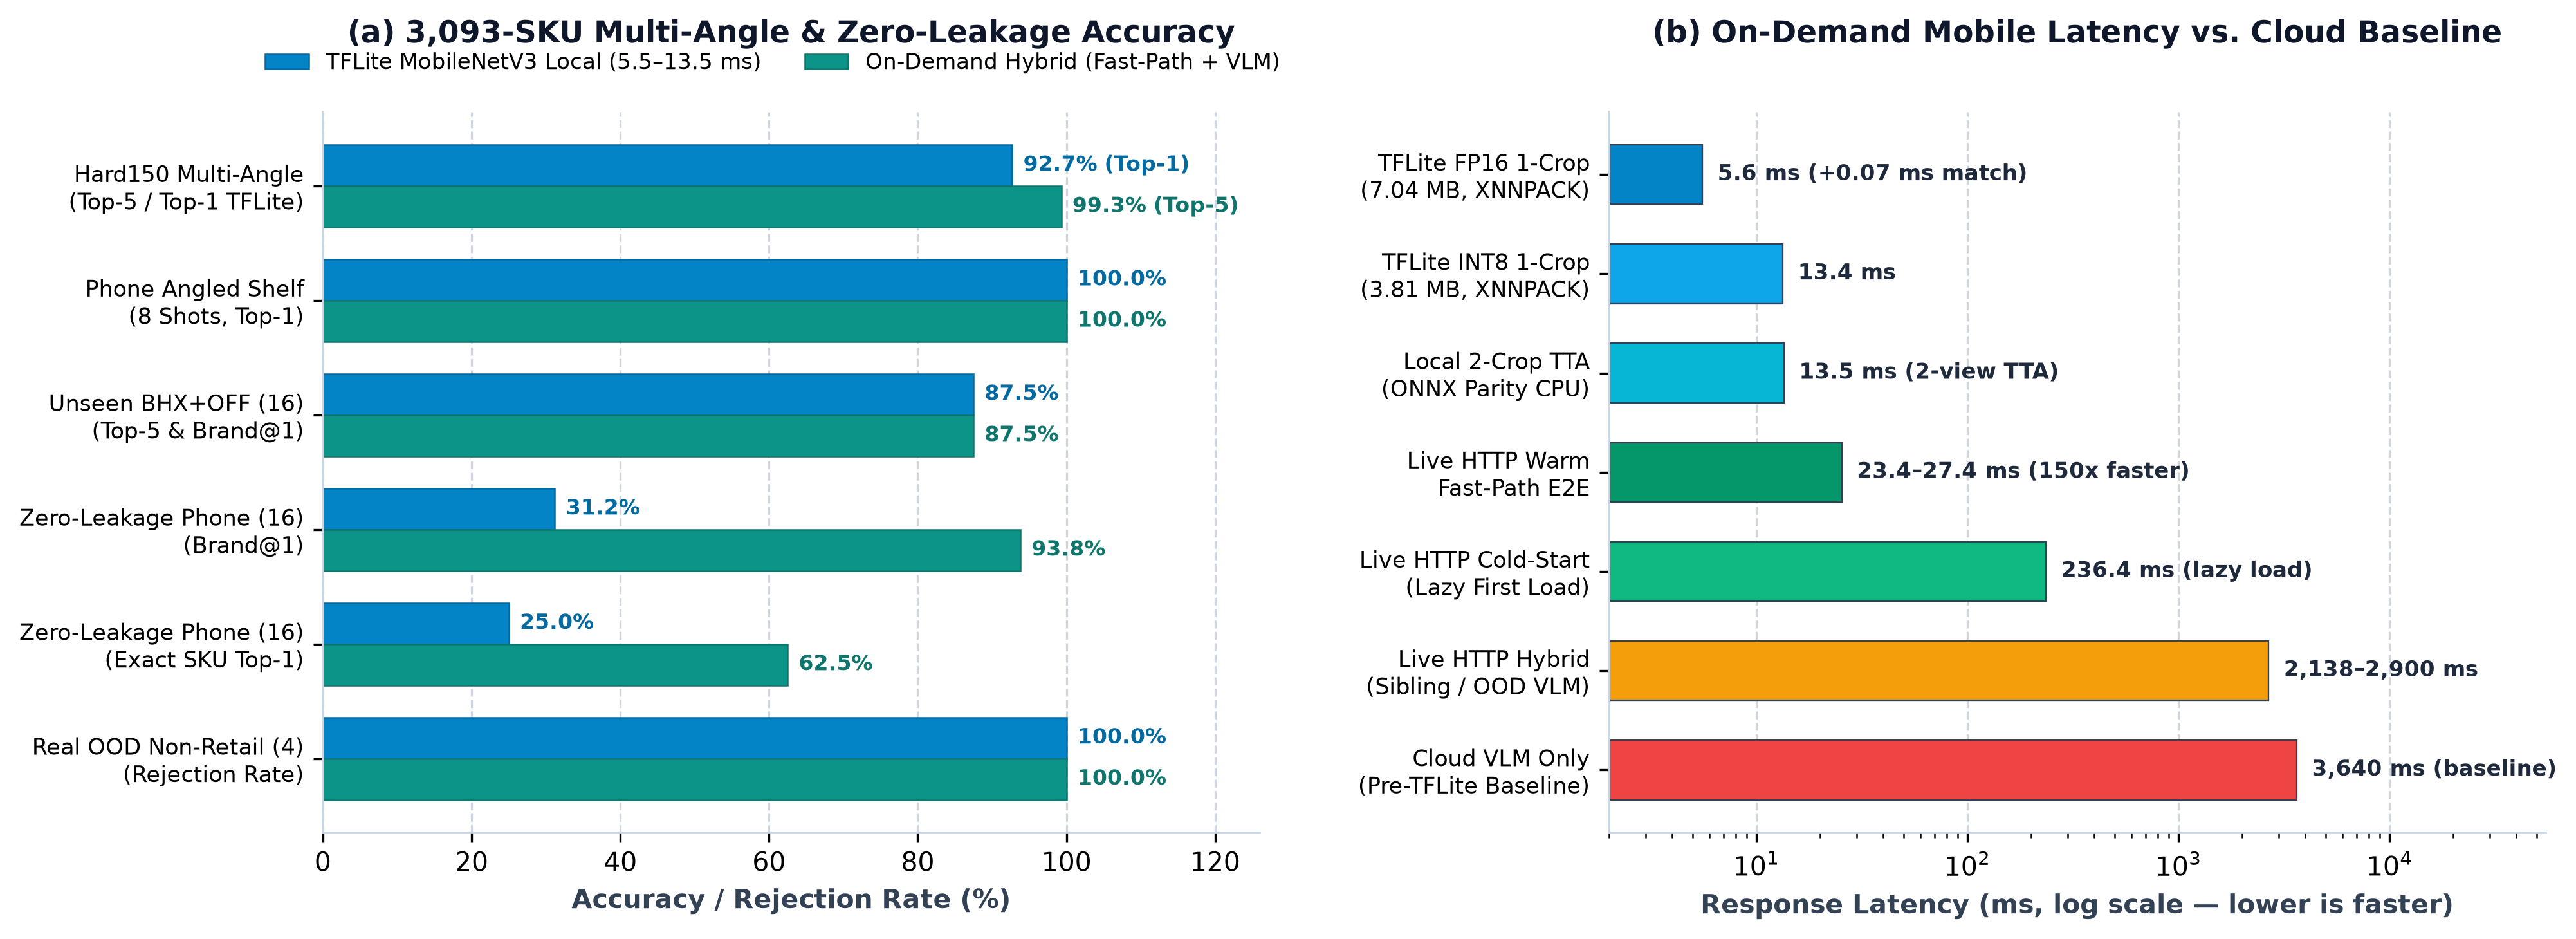
\includegraphics[width=0.98\textwidth]{Images/fig_mobile_tflite_vision.png}
    \caption{Độ chính xác nhận diện 3.093 SKU đa góc chụp và zero-leakage (trái) cùng so sánh độ trễ đầu-cuối theo thang log của mô hình \texttt{MobileNetV3Large-224} TFLite Fast-Path so với VLM đám mây (phải).}
    \label{fig:mobile_tflite_vision}
\end{figure}

\subsection*{Dự báo Hàng Tươi sống, Backtest Lợi nhuận 50 Cửa hàng và Kiểm toán Guard (\texttt{ops\_chest})}
Trên bộ dữ liệu FreshRetailNet-50K, bước khôi phục nhu cầu đứt hàng theo giờ hạ sai số WAPE từ \textbf{32,3\% xuống 20,5\%} và triệt tiêu gần như hoàn toàn thiên lệch âm (\textbf{$-32{,}3\% \to -0{,}1\%$}, $n=200.000$). Đánh giá trên 11.037 điểm đủ hàng, LightGBM~v3 hạ WAPE dự báo từ \textbf{35,1\% (EWMA) xuống 30,2\%}, giảm độ lệch từ \textbf{+6,9\% xuống +2,7\%} và đạt độ phủ thực nghiệm \textbf{81\%} cho khoảng dự báo danh định 80\% (so với 73\% của EWMA).

Tuy nhiên, kết quả backtest lợi nhuận A/B ngoài mẫu trong 37 ngày trên \textbf{50 cửa hàng độc lập} (kiểm định chéo 2 nếp, Bảng~\ref{tab:ops_chest_backtest} và Hình~\ref{fig:ops_chest_frn}) cho thấy một phát hiện thực nghiệm rất quan trọng: WAPE thấp hơn \emph{không tự động} mang lại lợi nhuận cao hơn:
\begin{itemize}
    \item Dùng thẳng \texttt{B-ML} (lấy độ rộng khoảng phân vị đối xứng của LightGBM làm độ lệch chuẩn) chỉ tăng +3,6\% so với Baseline~A---\emph{thua} \texttt{B-EWMA} (+4,2\%) tới $-0{,}4\%$ lợi nhuận trung vị và lỗ tới $-5{,}6\%$ ở các cửa hàng nhỏ ($\le 30$ SKU) vì độ phân tán đuôi nhiễu làm tỷ lệ hủy hàng tăng lên 5,7\%.
    \item Biến thể \texttt{B-ML split} bất đối xứng còn kém hơn (+1,6\% so với A, tỷ lệ hủy 6,5\%, chỉ thắng EWMA ở 6\% cửa hàng).
    \item Ghép trung vị điểm chính xác của LightGBM ($\hat{q}_{50}$) với độ lệch chuẩn mượt của EWMA ($\sigma_{\text{EWMA}}$) kết hợp cổng định tuyến lợi nhuận ngoài mẫu (\textbf{\texttt{B-Gate}}, \code{size_cut=30}) đạt hiệu quả vượt trội nhất: tăng \textbf{+4,9\% lợi nhuận cửa hàng} so với Baseline~A (\textbf{+0,8\%} trung vị so với \texttt{B-EWMA}, thắng trên \textbf{76\%} cửa hàng kiểm định), đạt \textbf{tỷ lệ hủy hàng thấp nhất (4,8\%)} và cắt giảm \textbf{61\% tình trạng đứt hàng nhóm hút khách} (từ 8,7\% xuống \textbf{3,4\%}). Trên Cửa hàng mẫu 18 (164 SKU tươi), \texttt{B-Gate} đạt +4,5\% lợi nhuận so với Baseline~A.
\end{itemize}

\begin{table}[H]
\centering
\caption{Backtest lợi nhuận A/B ngoài mẫu 37 ngày trên 50 cửa hàng FreshRetailNet-50K (2-fold CV)}
\label{tab:ops_chest_backtest}
\footnotesize
\setlength{\tabcolsep}{4pt}
\begin{tabularx}{\textwidth}{Y r r r r r r}
\toprule
\textbf{Chiến lược} & \textbf{Lãi vs.A} & \textbf{vs.EWMA} & \textbf{Thắng} & \textbf{Hủy\%} & \textbf{OOS\%} & \textbf{Traffic OOS\%} \\
\midrule
Baseline A (Giảm 30\% tối) & 0,0\% & --- & --- & 5,3 & 14,5 & 8,7 \\
\texttt{B-EWMA} (Ops Chest EWMA) & +4,2\% & 0,0\% & --- & 5,2 & 13,6 & 3,9 \\
\texttt{B-ML} (LightGBM \code{sym} $\sigma$) & +3,6\% & $-0{,}4\%$ & 38\% & 5,7 & 13,1 & 2,7 \\
\texttt{B-ML split} (split-normal $\sigma$) & +1,6\% & $-2{,}2\%$ & 6\% & 6,5 & \textbf{12,2} & \textbf{2,3} \\
\texttt{B-ML ewma\_sigma} (mọi SKU) & +4,5\% & +0,8\% & 74\% & \textbf{4,8} & 14,3 & 3,4 \\
\textbf{\texttt{B-Gate} (Cổng Lợi nhuận)} & \textbf{+4,9\%} & \textbf{+0,8\%} & \textbf{76\%} & \textbf{4,8} & 14,1 & \textbf{3,4} \\
\bottomrule
\end{tabularx}
\end{table}

\begin{figure}[H]
    \centering
    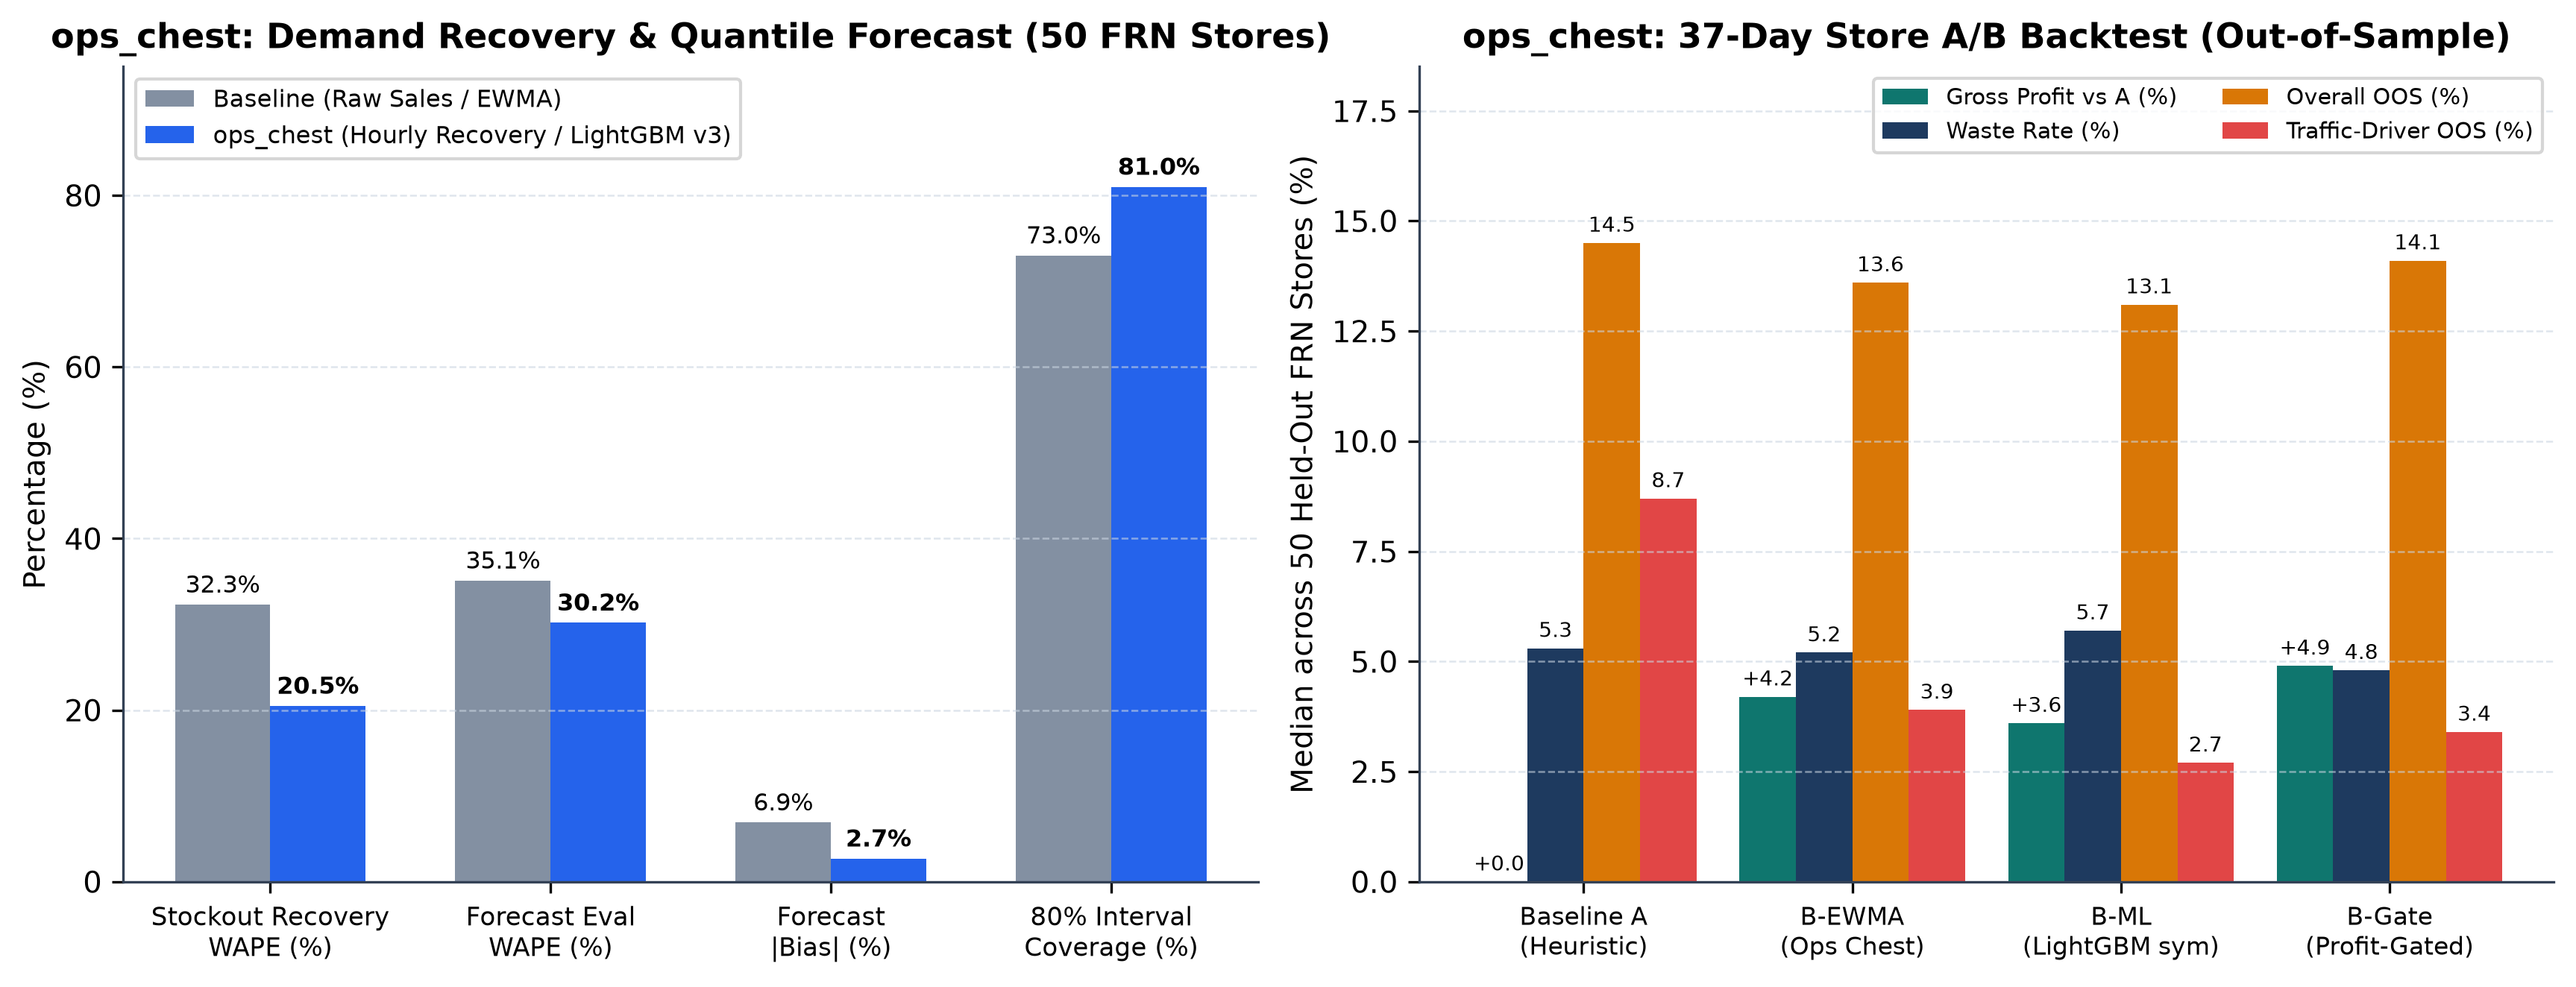
\includegraphics[width=0.98\textwidth]{Images/fig_ops_chest_frn_forecast.png}
    \caption{Kết quả thực nghiệm \texttt{ops\_chest} trên FreshRetailNet-50K: khôi phục nhu cầu và WAPE LightGBM~v3 (trái) cùng backtest lợi nhuận, hủy hàng và đứt hàng 50 cửa hàng (phải).}
    \label{fig:ops_chest_frn}
\end{figure}

Song song đó, Bảng~\ref{tab:ops_chest_guard} tổng kết kết quả 20 kịch bản kiểm định chuyển dự phòng đa nhà cung cấp và kiểm soát số liệu thời gian thực (\code{eval_failover.json}) của tác nhân vận hành \texttt{ops\_chest}.

\begin{table}[H]
\centering
\caption{Kiểm định gọi công cụ, căn cứ số liệu và an toàn HITL của \texttt{ops\_chest} (\code{eval_failover.json}, $N=20$)}
\label{tab:ops_chest_guard}
\footnotesize
\begin{tabularx}{\textwidth}{L{5.0cm} r r Y}
\toprule
\textbf{Tiêu chí An toàn / Chất lượng} & \textbf{Đạt} & \textbf{Tỷ lệ} & \textbf{Phạm vi Kiểm chứng} \\
\midrule
Căn cứ Số liệu (\code{grounded}) & 20 / 20 & \textbf{100,0\%} & Mọi con số $\ge 1.000$ đều khớp đầu ra công cụ hoặc câu hỏi \\
Chọn Đúng Công cụ (\code{tools_ok}) & 19 / 20 & 95,0\% & Gọi đúng công cụ đọc/đề xuất trong tập 31 công cụ \\
Không Nhận vơ Thực thi (\code{no_false_exec}) & 19 / 20 & 95,0\% & Tác nhân nêu rõ trạng thái \texttt{PENDING}, không tự nhận đã gửi \\
Đạt Nghiêm ngặt Toàn kịch bản & 18 / 20 & 90,0\% & Thỏa đồng thời căn cứ số, công cụ, ranh giới từ chối và định dạng \\
\bottomrule
\end{tabularx}
\end{table}

\section{Kết quả Định tính}

\subsection*{Giao diện Kiosk Giọng nói Trực tiếp (\texttt{Retail-AI-})}
Hình~\ref{fig:kiosk_live_ui} ghi lại màn hình vận hành trực tiếp của kiosk \texttt{Retail-AI-} trên trình duyệt Chrome trong phiên kiểm thử đầu-cuối, hiển thị avatar 2D tiếng Việt \emph{Mai}, bảng điều khiển giọng nói thời gian thực, câu trả lời có căn cứ và thẻ sản phẩm Thanh Lam Mart kèm giá VND chính xác.

\begin{figure}[H]
    \centering
    \includegraphics[width=0.95\textwidth]{Images/kiosk_live_ui.png}
    \caption{Giao diện trực tiếp của kiosk giọng nói \texttt{Retail-AI-} trên màn hình lớn hiển thị avatar \emph{Mai}, nội dung tư vấn tiếng Việt có căn cứ và thẻ sản phẩm Thanh Lam Mart.}
    \label{fig:kiosk_live_ui}
\end{figure}

Trên thiết bị di động ($390\times 844$\,px tại \url{https://mai-retail-kiosk.vercel.app}), Hình~\ref{fig:mobile_popup_live} minh họa tính năng mới \textbf{popup lightbox xem ảnh sản phẩm} được xác minh trực tiếp trên Production sau khi khách hỏi \emph{``Tương ớt Chin Su chai 1kg thành phần chính là gì v''} và chạm vào thẻ sản phẩm: hộp thoại hiển thị giữa màn hình với ảnh chai tương ớt rõ nét trên nền trắng ($299\times 299$\,px), nhãn thương hiệu \texttt{CHIN-SU}, ngành hàng, giá tham khảo 62.200\,đ/Chai, số lượng đã bán mô phỏng 284/30 ngày, nút \emph{``Hỏi thành phần''} và nút đóng sạch gọn, 0 lỗi console hay tràn khung.

\begin{figure}[H]
    \centering
    \includegraphics[width=0.42\textwidth]{Images/mobile_product_popup_live.png}
    \caption{Ảnh chụp trực tiếp trên di động Production ($390\times 844$\,px, \url{https://mai-retail-kiosk.vercel.app}) khi bấm vào thẻ sản phẩm \emph{Tương ớt Chin Su chai 1kg}: mở popup lightbox ảnh độ phân giải cao kèm giá, số liệu bán thử và nút hỏi nhanh thành phần.}
    \label{fig:mobile_popup_live}
\end{figure}

Năm tình huống hội thoại đã kiểm chứng minh họa rõ cách \texttt{Retail-AI-} xử lý bài toán thực tế tại siêu thị:
\begin{enumerate}
    \item \textbf{Minh bạch dữ liệu bán chạy kèm khẩu ngữ (\emph{``Ba chỉ bò Mỹ ACEFOODS loại nào bán chạy nhất?''} \& \emph{``cái nào bán chạy nhất v''}):} Thay vì bịa hạng bán chạy hoặc giả mạo dữ liệu mô phỏng thành POS thực, Mai giữ ngữ cảnh ngành hàng đang xem, lọc các tiểu từ khẩu ngữ (\emph{v, vậy, z, nhỉ}), xếp hạng xác định trên \code{demo_sales.sqlite3} ($\approx 212$\,ms), công bố rõ đây là số liệu minh họa 30 ngày và kèm đơn giá quy đổi.
    \item \textbf{Lắp giỏ món ăn đúng ngân sách dưới 1 giây (\emph{``Gợi ý bữa tối dưới 150k cho 2 người''}):} Nhánh đa món Path~E sử dụng \code{fast_chat()} trên Groq LPU tại Singapore (\texttt{sin1}) hoàn tất toàn bộ câu trả lời HTTPS kèm 4 thẻ thực phẩm mặn hợp lý chỉ trong \textbf{870\,ms} (rút từ 5,50\,s trước tối ưu), giữ nhất quán đại từ \emph{mình/bạn} và 100\% không vượt ngân sách.
    \item \textbf{Trả lời bảng thành phần định lượng \& xem ảnh tức thì (\emph{``Tương ớt Chin Su chai 1kg thành phần chính là gì v''}):} Tra cứu 0-token từ kho tri thức đã làm sạch 8 tầng trả đầy đủ \emph{``Nước, đường, ớt 110\,g/kg, muối, chất làm dầy (1422), tỏi, cà chua cô đặc...''} kèm thẻ có ảnh thu nhỏ mở popup lightbox phóng to sản phẩm khi chạm.
    \item \textbf{Báo quản lý thời gian thực qua Zalo Bot thân thiện người dùng:} Khi khách bấm \emph{Gọi quản lý · Zalo} hoặc nhờ gọi nhân viên, hệ thống đẩy cảnh báo trực tiếp qua Zalo Bot tới cửa hàng trưởng trong khi chỉ hiển thị thông báo tự nhiên cho khách hàng (ẩn toàn bộ mã UUID nội bộ và chuỗi trạng thái kỹ thuật như \code{NOTIFIED_ZALO}).
    \item \textbf{Phân biệt ranh giới y tế và câu hỏi vô hại:} Yêu cầu kê đơn thuốc điều trị bệnh (\emph{``thuốc hạ sốt trị đau dạ dày''}) bị chặn tức thì bằng thông điệp khuyến nghị gặp dược sĩ/bác sĩ, trong khi câu hỏi siêu thị vô hại chứa từ khóa nhạy cảm (XSTest 10/10, ví dụ \emph{``nước muối sinh lý súc miệng''} hoặc \emph{``trà gừng uống ấm bụng''}) được tư vấn tự nhiên không từ chối oan.
\end{enumerate}

\subsection*{Trợ lý Vận hành cho Cửa hàng trưởng (\texttt{ops\_chest})}
Trong phiên kiểm thử trên Cửa hàng mẫu 18 (164 SKU tươi sống), \texttt{ops\_chest} thể hiện bốn năng lực vận hành cốt lõi:
\begin{enumerate}
    \item \textbf{Bản tin Buổi sáng \& Đề xuất Giảm giá FEFO:} Khi kiểm tra rủi ro trong ngày, tác nhân gọi công cụ tổng hợp tồn kho và lô cận hạn, khoanh vùng các lô còn 1--2 ngày HSD có lượng tồn vượt sức bán nguyên giá, tính mức giảm giá bảo toàn lãi đóng góp dương và tạo đề xuất \texttt{PENDING} chờ duyệt.
    \item \textbf{Kiểm tra HSD bằng Vision OCR:} Khi tải ảnh nhãn gói thực phẩm tươi, \code{vision.py} trích xuất ngày hết hạn và số lượng lô rồi tự điền vào biểu mẫu kiểm HSD nội tuyến thay vì âm thầm sửa tồn kho.
    \item \textbf{Quản trị HITL \& Chặn Nhận vơ Thực thi:} Khi quản lý yêu cầu ``đặt ngay 50 gói từ nhà cung cấp X'', tác nhân chỉ gọi \code{propose_po}, giữ đơn ở trạng thái \texttt{PENDING} và thông báo rõ đơn email (Mailpit/SMTP) cần bấm duyệt; nếu LLM phát ngôn sai rằng đơn đã gửi, \code{guard.py} phát hiện ngay lỗi \code{FALSE_EXEC}.
    \item \textbf{Khép vòng Giả thuyết \& Học Thói quen Quản lý:} Cửa hàng trưởng có thể ghi nhận giả thuyết vận hành (như trời mưa cuối tuần làm giảm cầu nước giải khát) qua \code{propose_hypothesis} để hệ thống tự chấm kết luận sau chu kỳ (\code{hypotheses.py}), trong khi \code{edit_learning.py} theo dõi các chỉnh sửa lặp lại của quản lý để gợi ý điều chỉnh tinh hơn về sau.
\end{enumerate}

\section{Phân tích Lỗi và Thảo luận}

Việc mổ xẻ các trường hợp thất bại trên cả hai kho mã nguồn đã chỉ ra năm nguyên nhân gốc rễ quyết định kiến trúc cuối cùng và bộc lộ rõ các đánh đổi kỹ thuật còn tồn tại:
\begin{enumerate}
    \item \textbf{Vì sao ML có WAPE thấp hơn lại làm giảm lợi nhuận nếu thiếu Cổng Lợi nhuận (\texttt{ops\_chest}):} Phát hiện sâu sắc nhất trong \texttt{ops\_chest} là dù LightGBM~v3 hạ WAPE đi 4,9 điểm phần trăm (35,1\% $\to$ 30,2\%), nó lại \emph{làm lỗ} lợi nhuận ($-0{,}4\%$ trung vị chung và $-5{,}6\%$ ở cửa hàng $\le 30$ SKU) khi dùng chính khoảng phân vị $(q_{90}-q_{10})$ để tính tồn kho an toàn Newsvendor. Do cây phân vị trên chuỗi hàng tươi ngắn dễ phóng đại phương sai đuôi ở SKU bán thưa, việc thay bằng độ lệch chuẩn mượt $\sigma_{\text{EWMA}}$ và chặn ML ở cửa hàng nhỏ (\texttt{B-Gate}) đã đảo ngược từ lỗ $-0{,}4\%$ thành lãi \textbf{+0,8\%} so với EWMA (+4,9\% so với Baseline~A).
    \item \textbf{Lỗi dịch chuyển đặc trưng ở các phiên bản dự báo đầu (\texttt{ops\_chest}):} Phiên bản LightGBM~v1 đưa biến giảm giá ngày mục tiêu vào mô hình; do khuyến mãi tương lai chưa biết tại thời điểm dự báo (mặc định bằng 0), mô hình bị thiên lệch dự báo thấp tới $-15{,}7\%$. Tương tự, phép khử co giãn giá ở v2 ($e \approx 9{,}6$) gây sai lệch 14--31\%. Loại bỏ biến tương lai không quan sát được và neo v3 vào EWMA 56 ngày đã xóa sạch hai nguồn lệch này.
    \item \textbf{6/100 ca chưa đạt chuẩn nghiêm ngặt trên SOTA~V2 (\texttt{Retail-AI-}):} Trong 6 ca lỗi nghiêm ngặt (4 ca chức năng), 2 ca xuất phát từ việc CSV Thanh Lam Mart thiếu bảng thành phần dị ứng/dinh dưỡng chuẩn (buộc hệ thống từ chối khẳng định chắc chắn thay vì đoán bừa), 2 ca dùng từ lóng vùng miền quá hiếm ngoài bộ đồng nghĩa, và 2 ca yêu cầu so sánh đa thuộc tính kết hợp quy đổi gói phức tạp.
    \item \textbf{Đánh đổi giữa tuyến nhanh Groq LPU và lập kế hoạch JSON sâu trên đám mây (\texttt{Retail-AI-}):} Trong khi định tuyến lai Groq LPU + bộ đệm ngữ nghĩa + vùng Singapore (\texttt{sin1}) đã rút ngắn truy vấn đơn lạnh xuống \textbf{508--554\,ms}, giỏ bữa tối $<150\text{k}$ xuống \textbf{870\,ms} và cache xuống \textbf{125--140\,ms} với chi phí \$0, các kịch bản có lược đồ \code{json_schema} phức tạp (tư vấn dị ứng đa điều kiện hoặc làm rõ ngữ cảnh sâu) vẫn cần định tuyến về DeepSeek đám mây (1,3--2,0\,s) nhằm tránh vượt trần 8k TPM của gói miễn phí Groq. Triển khai mô hình tiếng Việt lượng tử hóa tại chỗ (vLLM) sẽ giúp đồng nhất độ trễ dưới 500\,ms cho cả hai nhánh.
    \item \textbf{2/20 ca biên trong đánh giá failover \texttt{ops\_chest}:} Trong \code{eval_failover.json}, 1/20 kịch bản bỏ sót một công cụ đọc phụ khi chuyển sang mô hình dự phòng yếu hơn và 1 ca diễn đạt sát biên kích hoạt cảnh báo \code{FALSE_EXEC}---càng khẳng định việc loại bỏ hoàn toàn công cụ tự thực thi khỏi lược đồ LLM là lớp phòng thủ cốt lõi không thể thay thế bằng prompt.
    \item \textbf{Giới hạn tự nhiên của ảnh nhúng $224\times 224$ với các mã hàng đồng mẫu khác dung tích (\texttt{Retail-AI-}):} Dù \texttt{MobileNetV3Large-224} TFLite đạt 92,67\% Top-1 trên ảnh đa góc nghiêng và 87,5\% Top-5/Brand@1 trên ảnh ngoài catalog chỉ trong 5,5--13,5\,ms, độ phân giải $224\times 224$ không đủ để đọc chữ định lượng nhỏ khi hai SKU dùng chung hệt một thiết kế bao bì (như \emph{Bơ Tường An 80\,g vs.\ 200\,g} hay \emph{TH True Milk ít đường vs.\ nguyên chất}). Bổ sung \emph{Cổng Bảo vệ Quy cách Anh em} đã triệt tiêu hoàn toàn lỗi chốt nhầm size trên nhánh Fast-Path bằng cách chuyển riêng các ca đồng dòng sang Hybrid VLM trong khi vẫn giữ tốc độ 23--27\,ms cho các SKU đặc trưng.
\end{enumerate}
